\documentclass{standalone}
\usepackage[utf8]{inputenc}
\usepackage[T1]{fontenc}
\usepackage{graphicx}
\usepackage{amsmath}
\usepackage[american,siunitx]{circuitikz}
\usetikzlibrary{arrows,shapes,calc,positioning}
\usepackage{tikzsymbols}
\usepackage{gensymb}
\usepackage{pgfplots}
\usepgfplotslibrary{groupplots}

\definecolor{mblue}{rgb}{0, 0, 0.7}
\definecolor{mred}{rgb}{0.7, 0, 0}
\definecolor{mgreen}{rgb}{0.1, 0.5, 0.0}
\definecolor{morange}{rgb}{0.8, 0.3, 0}

\begin{document}
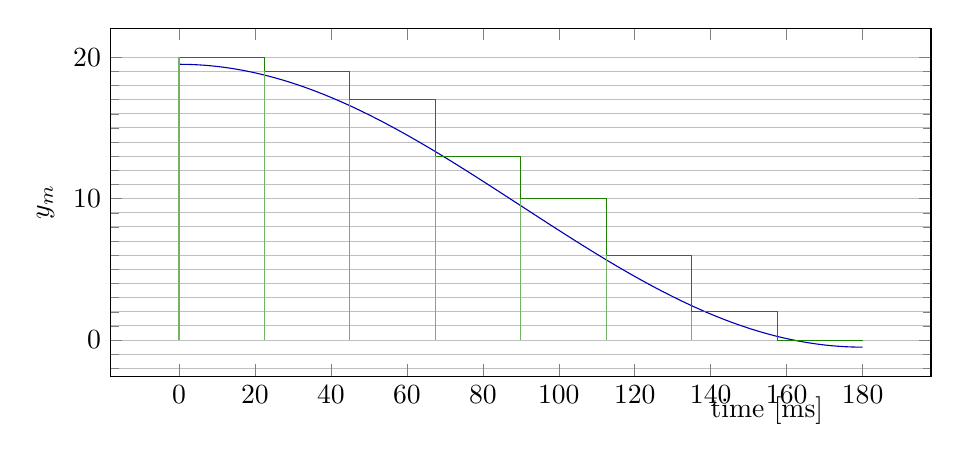
\begin{tikzpicture}[yscale=1,]
  \begin{axis}[
    clip=false,
    width=12cm,
    height=6cm,
    ylabel={$y_m$}, every major grid/.style={gray, opacity=0.5},
    yminorgrids,
    ymajorgrids,
    minor y tick num=9,
    x label style={at={(axis description cs: 0.8, -0.03)},anchor=north},
    xlabel={time [ms]},
    ]
    \addplot[mblue, no marks, domain=0:180, samples=180] {9.5+10*cos(x)};
    \addplot[mgreen, const plot, domain=0:180, samples=9] {round((9.5+10*cos(x))};
    \addplot[mgreen!60, ycomb, domain=0:180, samples=9] {round((9.5+10*cos(x))};
  \end{axis}
\end{tikzpicture}
\end{document}
